% !TEX encoding = UTF-8 Unicode

\documentclass[a4paper]{article}

\usepackage{color}
\usepackage{url}
\usepackage[T2A]{fontenc} % enable Cyrillic fonts
\usepackage[utf8]{inputenc} % make weird characters work
\usepackage{graphicx}

\usepackage[english,serbian]{babel}
%\usepackage[english,serbianc]{babel} %ukljuciti babel sa ovim opcijama, umesto gornjim, ukoliko se koristi cirilica

\usepackage[unicode]{hyperref}
\hypersetup{colorlinks,citecolor=green,filecolor=green,linkcolor=blue,urlcolor=blue}

%\newtheorem{primer}{Пример}[section] %ćirilični primer
\newtheorem{primer}{Primer}[section]

\begin{document}

\title{Naslov seminarskog rada\\ \small{Seminarski rad u okviru kursa\\Metodologija stručnog i naučnog rada\\ Matematički fakultet}}

\author{Uroš Milenković, Nikola Sojčić, Bojan Nestorović\\ enco164@gmail.com, soja.991@gmail.com,  bojants91@gmail.com}
\date{13.~april 2016.}
\maketitle

\abstract{
U ovom tekstu je ukratko prikazana osnovna forma seminarskog rada. Obratite pažnju da je pored ove .pdf datoteke, u prilogu i odgovarajuća .tex datoteka, kao i .bib datoteka korišćena za generisanje literature. Na prvoj strani seminarskog rada su naslov, apstrakt i sadržaj, i to sve mora da stane na prvu stranu! Kako bi Vaš seminarski zadovoljio standarde i očekivanja, koristite uputstva i materijale sa predavanja na temu pisanja seminarskih radova. Ovo je samo šablon koji se odnosi na fizički izgled seminarskog rada (šablon koji \emph{morate} da ispoštujete!) kao i par tehničkih pomoćnih uputstava. Molim Vas da kada budete predavali seminarski rad, imenujete datoteke tako da sadrže temu seminarskog rada, kao i imena i prezimena članova grupe (ili samo temu i prezimena, ukoliko je sa imenima predugačko). Predaja seminarskih radova biće isključivo preko web forme, a NE slanjem mejla.

\tableofcontents

\newpage

\section{Uvod}
\label{sec:uvod}

Lorem ipsum dolor sit amet, consectetur adipiscing elit. Praesent eu dui sed nulla gravida auctor. Phasellus cursus massa turpis, eu luctus mi sodales vitae. Mauris faucibus ut diam eu posuere. Lorem ipsum dolor sit amet, consectetur adipiscing elit. Aliquam in fringilla ex. Donec facilisis lectus quis velit mollis, sit amet pulvinar velit commodo. Cras hendrerit lectus id molestie venenatis. Phasellus quis mi erat. Praesent posuere augue at mauris porttitor cursus. Nam imperdiet libero iaculis, vehicula ipsum nec, malesuada libero.

Sed eu dictum ex. Aenean auctor tellus eget dictum cursus. Curabitur a tempus sapien, ut hendrerit metus. Quisque elit mauris, elementum id placerat et, vehicula eget nisl. Vestibulum ultrices euismod quam eu rhoncus. Integer vel dolor ac augue molestie consectetur. Donec feugiat pharetra consectetur. Cras dictum, augue non gravida auctor, ligula nunc hendrerit velit, vel vulputate est arcu sed velit. Lorem ipsum dolor sit amet, consectetur adipiscing elit.

Proin suscipit tempor massa, nec commodo urna posuere at. Vestibulum nec velit rhoncus, consequat velit eget, cursus leo. Morbi facilisis scelerisque sagittis. Nullam suscipit lobortis placerat. Praesent ullamcorper tempor purus aliquam suscipit. Nulla fringilla lobortis elit rhoncus cursus. Integer commodo vestibulum lacus vel dapibus. Integer sed quam malesuada libero efficitur interdum. Aliquam suscipit aliquam justo, eget tempus leo placerat quis. Cras tristique quis arcu vel mollis. Sed laoreet sem id enim auctor, eu pellentesque augue iaculis. Nullam viverra velit in efficitur dapibus. Donec sed cursus lacus.


\section{Build Jobs}

Build jobs predstavlja skup poslova u koji spadaju kompajliranje, testiranje, pakovanje, razvijanje projekta ili bilo koji drugi posao koji manevriše sa vašim projektom. Build job je osnovni pojam kad se govori o principu kontinualne integracije.

\subsection{Kreiranje Build Job-a}

Pravljenje build job-a je veoma jednostavno i ono podrazumeva razna podešavanja. Prvo treba odrediti kakvog će tipa biti projekat. Postoje četiri osnovne vrste i to su:
\begin{itemize}  
\item Slobodan projekat(Freestyle software project) - Vrsta projekta koji pružaju maksimalnu fleksibilnost i koji služe za osnovnu upotrebu
\item Maven project - buiild job koji je specijalno namenjen Maven projektima 
\item External job - ova opcija služi da se prate izvršavanja nekog drugog procesa koji se ne nalazi na Jenkins-u
\item Multi-configuration project - ova opcija je pogodna za projekte koji zahtevaju više različitih konfigurisanja
\item Copy existing job - projekat može da bude i kopija već postojećeg projekta koji zahteva neke promene u konfigurisanju
\end{itemize}  

\subsubsection{Kreiranje slobodnog projekta}

Slobodan projekat je najfleksibilnija vrsta i može se koristiti za bilo koju vrstu projekta. Puno opcija koje se nameštaju u okviru slobodnog projekta se javljaju i u ostalim vrstama projekta. Pri kreiranju projekta prvo se unose osnovni podaci kao što su ime projekta i opis projekta. Zatim slede opcije:

\begin{itemize}  
\item Discard Old Builds - čekiranjem ove opcije limitirate broj build-ova koji će se čuvati, postoje dva kriterijuma:
\begin{itemize}
\item Po starosti - build se briše posle određenog vremena
\item Po broju - čuva se N build-ova
\end{itemize}
\item This build is parameterized - korisnik dodeljuje parametre koje će build koristiti. Neki od parametara su:
\begin{itemize}
\item Boolean Parameter - definiše se string ''true'' ili ''false'' koji se može koristiti u procesu build-ovanja
\item Choice Parameter - definiše se string koji može imati bilo koju vrednost iz liste izbora i koji se može koristiti u procesu build-ovanja
\item Password Parameter - definiše se tekst gde korisnici mogu da unesu string vrednost koji se može koristiti tokom proces build-ovanja
\end{itemize}
\item Disable Build - kad je čekirano privremeno se obustavlja build-ovanje
\item Execute concurrent builds if necessary - čekiranjem ove opcije, omogućava se paralelno izvršavanje build-ovanja. Veoma kosrisno kod parametrizovanih build-ova gde su izvršavanja nezavisna jedna od drugih
\end{itemize}

''Napredne'' opcije:
\begin{itemize}  
\item Quiet period - čekiranjem ove opcije, zadaje se broj sekundi nakon koliko će se pokrenuti sledeći build
\item Retry Count - u slučaju da build ne uspe, zadaje se broj ponovnih pokušaja
\item Block build when upstream project is building - sprečava se build-ovanje ako je neki projekat koji je zavistan od njega isto u procesu build-ovanja
\item Block build when downstream project is building - sprečava se build-ovanje ako je neki projekat koji je ''dete'' isto u procesu build-ovanja
\item Use custom workspace - manualno zadavanje radnog prostora
\item Keep the build logs of dependencies
\end{itemize}

\subsection{Integracija sa izvornim kodom}

Jedna od najbitnijih i najznačajnijih stvari je integracija sa sistemom za kontrolu verzija. Jenkins prati svaku promenu u vašem izvornom kodu posle kojih se pokreće kompajliranje i razni automatski testovi. Podržani su razni sistemi za kontrolu verzija, CVS i Subversion ''u startu'', dok za sisteme kao što su Git, Mercurial, Harvest, BitKeeper i ostale postoje plugin-ovi koji se lako instaliraju preko Jenkins plugin Manager-a. Pri pravljenju projekta i odabiru koji sistem za kontrolu verzija će se koristiti, unošenjem URL-a repozitorijuma se vrši integracija sa izvornim kodom.

\subsection{Git Setup}

Da bismo mogli da se povežemo sa Git-om prvo moramo instalirati Git. Za operativne sisteme Windows i Mac OS postoje instalacije, a na Linuxu se instalira putem jednostavne komande:

\begin{verbatim}
 sudo apt-get install git-all
\end{verbatim}

Za razliku od sistema za kontrolu verzija kao što su CVS i Subversion čiji su plugin-ovi već instalirani, plugin za Git, koji se nalazi u Jenkins-ovom plugin Manager-u, morate sami instalirati. Nakon instalacije pri pravljenju novog projekta, u opcijama za biranje sistema za kontrolu verzija otvoriće se opcija i za Git što je prikazano na slici \ref{fig:git}

\begin{figure}[h!]
\begin{center}
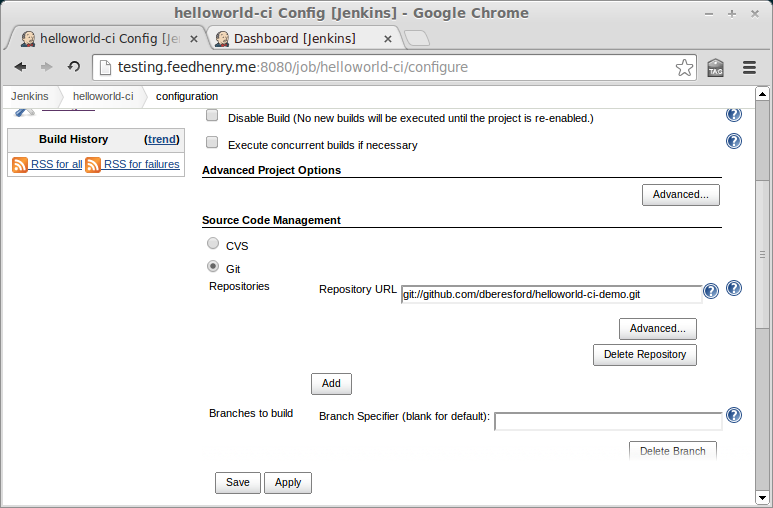
\includegraphics[scale=0.75, totalheight=0.4\textheight]{slike/git_jenkins.png}
\end{center}
\caption{Git}
\label{fig:git}
\end{figure}

Uz opcije ''Repository'' gde se navodi URL repozitorijuma i ''Branches to build'' gde se navodi ime branch-a(grane) koje se build-uje postoje je tzv. ''Dodatna ponašanja''(Additional Behaviours). Neka od njih su:
 
\begin{itemize}  
\item Polling ignores commits from certain paths
\begin{enumerate}
\item Included regions - unose se putanje fajlova koje se build-uju
\item Excluded regions - unose se putanje fajlova čije testiranje nema efekta npr. slike
\end{enumerate}
\item Polling ignores commits in certain users 
\begin{description}
\item Excluded users - imena user-a od čije strane ne može da se pokrene build-ovanje
\end{description}
\end{itemize}

\subsection{Pokretanje build-ova}

Nakon nameštanja koji ćete sistem za kontrolu verzija koristiti, vreme je da se konfiguriše kada će se build-ovi pokretati. Postoje osnovne tri vrste pokretanja build-ova, a to su:

\begin{itemize}
  
\item Build after other projects are built - ova opcija pruža pokretanje build-a kad god se neki drugi build izvrši. Postoje i 3 dodatne opcije:
\begin{itemize}  
\item Trigger only if build is stable - pokreni build samo ako je build stabilan
\item Trigger even if the build is unstable - pokreni build iako je build nestabilan
\item Trigger even if the build fails - pokreni build iako build ne uspe
\end{itemize}

\item Build periodically

Odlika kontinualne integracije jeste kontinualno izvršavanje build-ovanja nakon svake promene što nije stvar kod periodičnog build-ovanja. U nekim slučajevima je i pogodno koristiti ovu vrstu pokretanja npr. kod projekata gde iscrpna testiranja traju i po nekoliko sati i gde je pogodnije pokretati build-ove u određenim vremenskim intervalima.
Sintaksa za zadavanje vremenskog intervala: \\
MINUTE HOUR DOM MONTH DOW
\begin{itemize}
\item MINUTE - minut u satu (0-59)
\item HOUR - sat u danu (0-23)
\item DOM - dan u mesecu (1-31)
\item MONTH - mesec(1-12)
\item DOW - dan u nedelji(0-7) gde su 0 i 7 nedelje
\end{itemize}

\item Poll SCM

Bolja strategija od periodičnog build-ovanja jeste Polling the SCM tzv. ''ispitivanje'' sistema za kontrolu verzija. Ideja je da se sistem za kontrolu verzija ''ispituje'' da li je napravljena izmena u izvornom kodu. U slučaju da jeste Jenkins će pokrenuti build.
\end{itemize}

\subsection{Koraci build-ovanja}

Definisanjem build koraka govorite Jenkins-u šta da radi sa vašim izvornim kodom. Jedan build može da ima više koraka u koje spadaju izvršavanje shell skripte, izvršavanje Windows batch komande ili povezivanje sa Maven-om ili Ant-om.

\subsection{Akcije posle build-ovanja}

Nakon samog procesa build-ovanja potrebno je preduzeti neke akcije. Neke od mogućih akcija su:
\begin{itemize}
\item Archive the artifacts - ova opcija omogućava da se rezultati build-ovanja čuvaju u određenom formatu i da se zatim download-uju
\item E-mail Notifications - Jenkins obaveštava mejlom svaki put kada build ne uspe, kada uspe build nakon neuspelog pokušaja, kada je build nestabilan nakon uspešnog build-ovanja.
\end{itemize}

\section{Automatsko testiranje}
Jedna od bitnih aktivnost u ciklusu je automatsko testiranje softvera \cite{jenkins:2011}. Automatsko testiranje značajno unapređuje razvojni proces. Ovakvi testovi daju sigurnost da nove izmene u kodu neće pogoršati stabilnost sistema, kao i da će funkcionalnosti koje su do tada radile, nastaviti da rade. Timovi treba da ulažu u pisanje testova jer se njima podiže kvalitet proizvoda, a cena testiranja je mnogo manja u odnosu na kasnije ispravke. 

Najefikasniji pristup pisanja dobrih testova je da se testovi pišu na početku, pre pisanja samog k\^oda. Ovakva tehnika se naziva razvoj vođen testovima (eng.~{\em Test Driven Development}). U te svrhe se najčešće koriste testovi jedinica (eng.~{\em Unit tests}). 

U ovom poglavlju ćemo pokazati kako se u Jenkins može integrisati automatsko testiranje. Iako postoji mnogo različitih načina za testiranje softvera, držaćemo se uglavnom testova jedinica jer smatramo da je takav pristup testiranju najzastupljeniji.

\subsection{Uključivanje testova jedinica u proces}
Postoje različiti testovi jedinica za razne jezike. Najpoznatija grupa testova jedinica su \textit{x}Unit testovi, gde \textit{x} označava programski jezik (za Java programski jezik će biti JUnit, za PHP će biti PHPUnit itd.). 

\textit{x}Unit testovi kao rezultat testiranja generišu neku vrstu izveštaja u XML datoteku za koju se zna shema. To znači dve stvari. Prvo, da alati za testiranje ne moraju da budu baš iz \textit{x}Unit familije, već mogu biti bilo kakvi alati koji će svoj izveštaj generisati u XML datoteku. Drugo, da Jenkins može da parsira taj izveštaj i lepše da ga prikaže za razliku od XML datoteke.

Automatsko testiranje se izvršava kao jedna od operacija build procesa. Pošto je izlaz testiranja XML datoteka, jedino što preostaje da se uradi je da se konfiguraciji projekta postavi putanja do izlazne XML datoteke.

\subsubsection{Konfigurisanje test izveštaja i prikazivanje rezultata}
Prvo je potrebno dodati novu post-build akciju. Iz padajućeg menija treba izabrati "Publish JUnit test result report". Jenkins dolazi sa preinstaliranim dodatkom za JUnit test izveštaje. Ako je projekat testiran u nekom drugom \textit{x}Unit alatu, potrebno je instalirati plugin koji se zove "xUnit" i njega koristiti. Od konfiguracije build menadžera zavisi putanja XML izveštaja. Tu putanju upisujemo u polje "Test report XMLs", kao što je prikazano na slici \ref{fig:test_xml_path}. 

\begin{figure}[h!]
\begin{center}
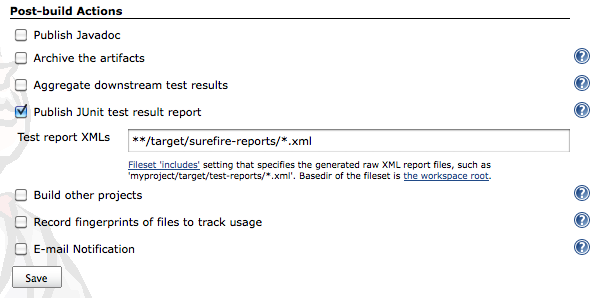
\includegraphics[scale=0.5]{slike/test_xml_path.png}
\end{center}
\caption{Podešavanje putanje za XML izveštaj}
\label{fig:test_xml_path}
\end{figure}

Kada je konfigurisan test izveštaj, Jenkins na početnoj strani projekta prikazuje grafikon na kome se mere za uspešne i neuspešne testove. Kao što se sa slike  \ref{fig:test_project_home} vidi, uspešni su obojeni plavom bojom, dok su neuspešni obojeni crvenom bojom. 

\begin{figure}
\begin{center}
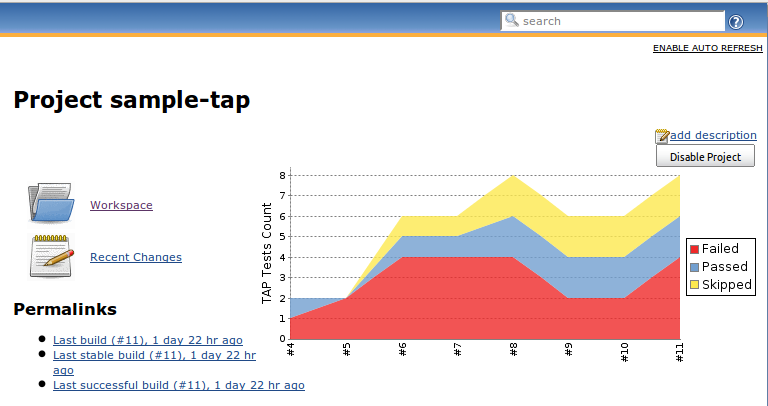
\includegraphics[scale=0.45]{slike/test_project_home.png}
\end{center}
\caption{Početna strana projekta sa izveštajem}
\label{fig:test_project_home}
\end{figure}

U sekciji sa linkovima na početnoj strani možemo videti poslednji build, poslednji stabilni build i poslednji uspešni build. Izborom linka za poslednji build prelazimo na ekran sa detaljima o tom buildu. Na slici \ref{fig:test_last_build} je prikazan ekran sa detaljima. U detaljima Jenkins nam prikazuje koji testovi nisu prosli. Klikom na link neuspešnog testa dobijamo ekran sa detaljima zašto određeni test nije prošao. Ovako se jednostavno fokusiramo na greške i možemo ih brže ispraviti.

\begin{figure}
\begin{center}
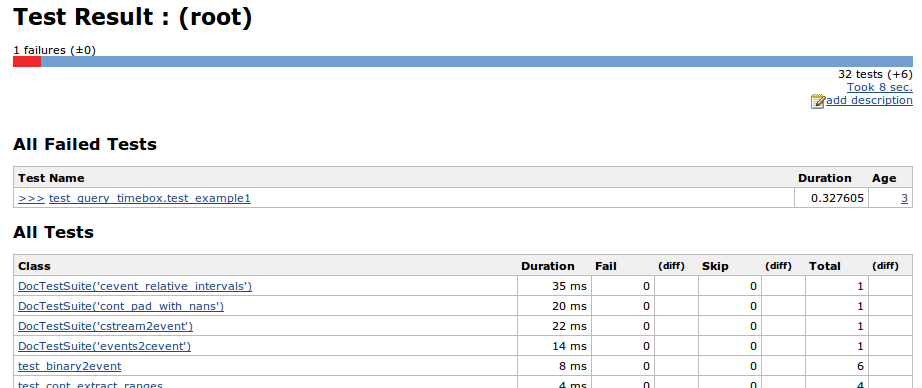
\includegraphics[scale=0.35]{slike/test_last_build.png}
\end{center}
\caption{Poslednji build sa izveštajem o testovima}
\label{fig:test_last_build}
\end{figure}

Testovi jedinica su dizajnirani tako da budu brzi. Na većim projektima testovi mogu da traju i po par sati, a nekada se oni pokreću i više puta dnevno. Spori testovi troše dragoceno vreme programera. Zato je veoma bitno da se testovi pišu tako da budu efikasni. U tu svrhu veoma je poželjno da imamo povratnu informaciju o tome koliko testovi dugo traju, kako bismo mogli da uvidimo problem. Srećom, Jenkins nam pruža lepu vizuelizaciju koliko dugo su se testovi izvršavali za svaki build. Na slici \ref{fig:buildtimetrend} je prikazan grafikon performansi build-ova koji uključuju testove.

\begin{figure}
\begin{center}
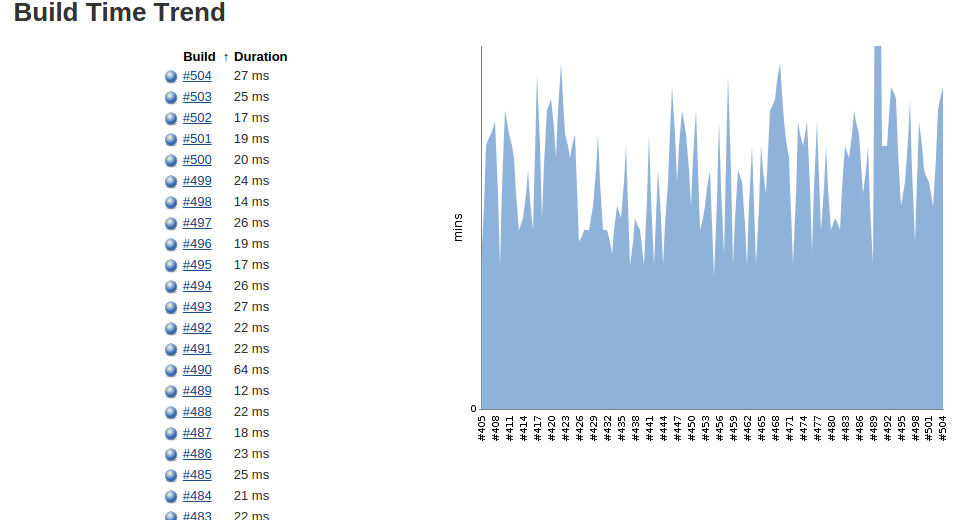
\includegraphics[scale=0.35]{slike/buildtimetrend.png}
\end{center}
\caption{Performanse build-ova}
\label{fig:buildtimetrend}
\end{figure}

\subsection{Pokrivenost k\^oda}
Jedna od metrika koja se ceni u testiranju softvera je \textit{pokrivenost k\^oda}. Iako ona ne daje neku značajnu informaciju o kvalitetu napisanog k\^oda, daje informaciju koliki deo k\^oda je pokriven testovima jedinica. Na primer, ako naši testovi za neku funkcionalnost uvek prolaze kroz \verb|if| granu ali ne i kroz \verb|else| granu.

Standardni alati za testiranje pružaju opcije za pregled pokrivenosti k\^oda u obliku generisanih HTML stranica. Prednost integracije ove metrike u Jenkins je što je možemo pratiti iz build-a u build kroz Jenkins. 

Kao i za većinu funkcionalnosti kod Jenkins sistema, potrebno je instalirati plug-in. Najpoznatiji alat za pokrivenost k\^oda za Javu je Cobertura koji se uključuje u build proces. Izlaz Cobertura alata je XML fajl do kojeg je potrebno da se podesi putanja u Jenkins-u. Tada Jenkins može da iz XML fajla napravi lepe grafikone i lepše prikaže ovu metriku.

Drugi alati, kao na primer PHPUnit, u sebi već imaju ugrađene sisteme za pokrivenost k\^oda. S toga, nije potrebno ništa dodatno podešavati jer plugin-ovi su dovoljno pametni da to prepoznaju i integrišu u Jenkins.

Na slici \ref{fig:test_project_coverage} je prikazano kako izgleda grafikon pokrivenosti k\^oda koji prikazuje Jenkins za ceo projekat. Na sledećoj slici REF možemo pogledati metriku vezanu za određeni paket, dok kad kliknemo na određenu klasu prikazaće nam se k\^od te klase sa obojenom pozadinom koja nam pokazuje koji to delovi k\^oda nisu a koji jesu pokriveni testovima.

\begin{figure}
\begin{center}
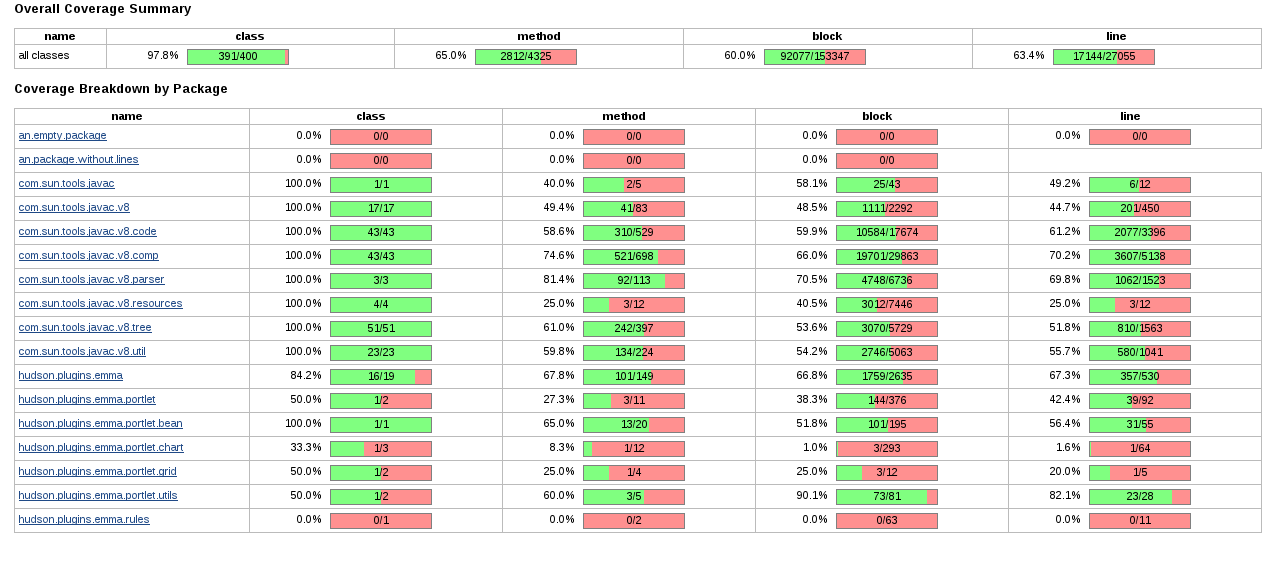
\includegraphics[scale=0.25]{slike/test_project_coverage.png}
\end{center}
\caption{Početna strana projekta sa izveštajem}
\label{fig:test_project_coverage}
\end{figure}





%Bojan nestorovic

\section{Deployment}

Postoje mnogi dodaci koji se koriste da prebace build fajlove posle uspesnog kompajliranja na željenu lokaciju ili web server. Ovde ćemo to pokazati na primeru "Deploy to container Plugin". 

\subsection{Instalacija dodatka Deploy to container Plugin}

Da bi se instalirao taj dodatak, potrebno je otići na Jenkins -> Manage Plugins, pronađete željeni dodatak i instalirate ga kao što je prikazano na slici \ref{fig:deploy_to_container_plugin}. Posle toga je potrebno restartovati jenkins server. Ovaj dodatak uzima fajlove i prebacuje ih automatski na server na kraju svakog builda.
\begin{figure}
\begin{center}
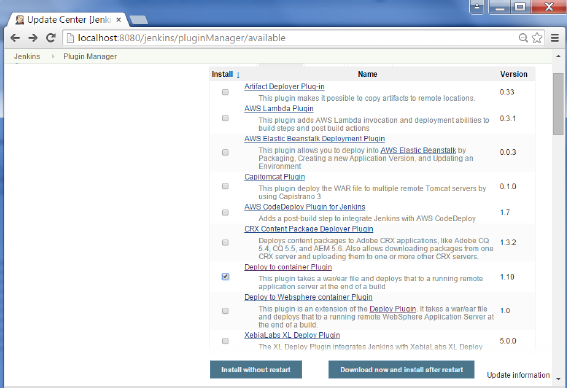
\includegraphics[scale=0.45]{slike/deploy_to_container_plugin.png}
\end{center}
\caption{Dodavanje dodatka}
\label{fig:deploy_to_container_plugin}
\end{figure}


\subsection{Podešavanje}

Potrebno je otici na Vaš Build project i kliknuti na Configure option. Izaberite opciju "Deploy war/ear to a container" kao što je prikazano na slici \ref{fig:deploy_war_ear_container}.

\begin{figure}
\begin{center}
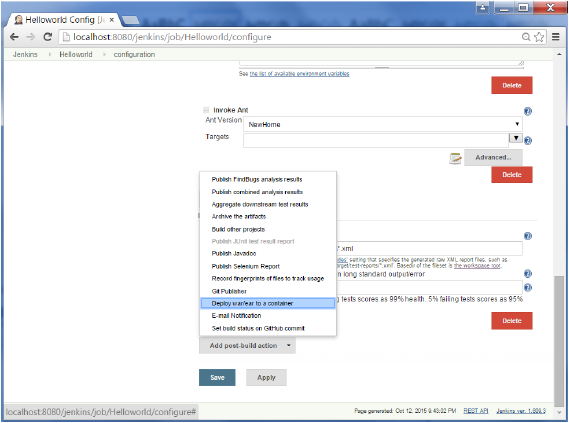
\includegraphics[scale=0.45]{slike/deploy_war_ear_container.png}
\end{center}
\caption{Deploy war/ear to a container dodatak}
\label{fig:deploy_war_ear_container}
\end{figure}

U polja prikazana na slici \ref{fig:demo_config.png} unesite detalja servera na kojem želite da se fajlovi šalju i kliknite na Save dugme. Ovi koraci će obezbediti da se potrebni fajlovi nadju na serveru posle uspešnog build-a.

\begin{figure}
\begin{center}
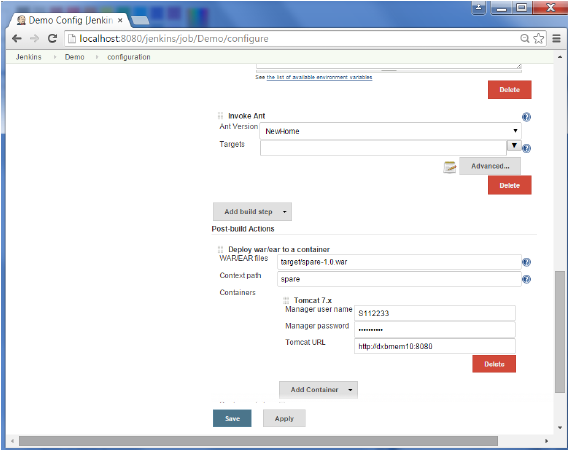
\includegraphics[scale=0.45]{slike/demo_config.png}
\end{center}
\caption{Konfigurisanje parametara}
\label{fig:demo_config.png}
\end{figure}





\section{Zaključak}
\label{sec:zakljucak}

Lorem ipsum dolor sit amet, consectetur adipiscing elit. Praesent eu dui sed nulla gravida auctor. Phasellus cursus massa turpis, eu luctus mi sodales vitae. Mauris faucibus ut diam eu posuere. Lorem ipsum dolor sit amet, consectetur adipiscing elit. Aliquam in fringilla ex. Donec facilisis lectus quis velit mollis, sit amet pulvinar velit commodo. Cras hendrerit lectus id molestie venenatis. Phasellus quis mi erat. Praesent posuere augue at mauris porttitor cursus. Nam imperdiet libero iaculis, vehicula ipsum nec, malesuada libero.

Sed eu dictum ex. Aenean auctor tellus eget dictum cursus. Curabitur a tempus sapien, ut hendrerit metus. Quisque elit mauris, elementum id placerat et, vehicula eget nisl. Vestibulum ultrices euismod quam eu rhoncus. Integer vel dolor ac augue molestie consectetur. Donec feugiat pharetra consectetur. Cras dictum, augue non gravida auctor, ligula nunc hendrerit velit, vel vulputate est arcu sed velit. Lorem ipsum dolor sit amet, consectetur adipiscing elit.


\addcontentsline{toc}{section}{Literatura}
\appendix
\bibliography{seminarski} 
\bibliographystyle{plain}

\appendix
\section{Dodatak}
Ovde pišem dodatne stvari, ukoliko za time ima potrebe.
Ovde pišem dodatne stvari, ukoliko za time ima potrebe.
Ovde pišem dodatne stvari, ukoliko za time ima potrebe.
Ovde pišem dodatne stvari, ukoliko za time ima potrebe.
Ovde pišem dodatne stvari, ukoliko za time ima potrebe.


\end{document}
